\documentclass[12pt,letterpaper]{article}

\usepackage[letterpaper,margin=1.2in]{geometry}
\usepackage{fancyhdr}
\usepackage{lastpage}
\usepackage{graphicx}
\usepackage{ragged2e}
\usepackage{csquotes}
\usepackage{url}
\usepackage{import}
\usepackage{color}
\usepackage[T1]{fontenc}
\usepackage{verbatim}
\usepackage{listings}
\definecolor{mygreen}{rgb}{0,0.6,0}
\definecolor{mygray}{rgb}{0.5,0.5,0.5}
\definecolor{mymauve}{rgb}{0.58,0,0.82}

\lstset{
    basicstyle=\scriptsize,
    numbers=left,
    numberstyle=\scriptsize,
    stepnumber=5,
    numbersep=5pt,
    showspaces=false, % don't show spaces by adding underscores
    showstringspaces=false, % don't underline spaces in strings
    showtabs=false, % don't show tabs with underscores
    frame=single,
    tabsize=4,
    captionpos=b,
    breaklines=true,
    breakatwhitespace=false,
    numberbychapter=false,
    stringstyle=\ttfamily %typewriter type for strings
      captionpos=b,                    % sets the caption-position to bottom
  commentstyle=\color{mygreen},    % comment style
  escapeinside={\%*}{*)},          % if you want to add LaTeX within your code
  keywordstyle=\color{blue},       % keyword style
  stringstyle=\color{mymauve},     % string literal style
}
\lstdefinelanguage{JavaScript}{
  keywords={break, case, catch, continue, debugger, default, delete, do, else, false, finally, for, function, if, in, instanceof, new, null, return, switch, this, throw, true, try, typeof, var, void, while, with},
  morecomment=[l]{//},
  morecomment=[s]{/*}{*/},
  morestring=[b]',
  morestring=[b]",
  ndkeywords={class, export, boolean, throw, implements, import, this},
  keywordstyle=\color{blue}\bfseries,
  ndkeywordstyle=\color{darkgray}\bfseries,
  identifierstyle=\color{black},
  commentstyle=\color{purple}\ttfamily,
  stringstyle=\color{red}\ttfamily,
  sensitive=true
}
\lstdefinelanguage{json}{
  showstringspaces    = false,
  keywords            = {false,true},
  alsoletter          = 0123456789.,
  morestring          = [s]{"}{"},  
}


\setlength{\headheight}{15pt}
\topmargin=-0.45in
\evensidemargin=0in
\oddsidemargin=0in
\textwidth=6.5in
\textheight=9.0in
\headsep=0.25in
\linespread{1.0}
\pagestyle{fancy}
\rhead{\AssShortTitle}
\lhead{\Class\ (\Instructor\ \Semster)}
\lfoot{}
\cfoot{\thepage}
\rfoot{}
\renewcommand\headrulewidth{0.4pt}
\renewcommand\footrulewidth{0.4pt}

\newcommand{\AssignmentTitle}{Assignment\ 6}
\newcommand{\Class}{CS532 Web Science}
\newcommand{\Instructor}{Dr. Michael L. Nelson}
\newcommand{\Semster}{- Spring 2016}
\newcommand{\AssShortTitle}{Assignment 6}
\newcommand{\MyName}{Naina Sai Tipparti}
\newcommand{\MyEmail}{ntippart@cs.odu.edu}

\setcounter{secnumdepth}{0}

\title{
\vspace{2in}
\textmd{\textbf{\Class:\ \AssignmentTitle}}\\
\normalsize\vspace{0.1in}\small{Finished on \today}\\
\vspace{0.1in}\large{\textit{\Instructor\ }}
\vspace{3in}
}

\author{\textbf{\MyName} \\ \MyEmail}
\date{}

\begin{document}
\begin{titlepage}
\clearpage\maketitle
\thispagestyle{empty}
\end{titlepage}


\newpage
\clearpage
\tableofcontents
\lstlistoflistings
\listoffigures
\thispagestyle{empty}

\section{Problem 1}

\subsection{Question}
\vspace*{10pt}
Write a Python program that extracts 1000 unique links from
Twitter.  You might want to take a look at:\\
\\
http://thomassileo.com/blog/2013/01/25/using-twitter-rest-api-v1-dot-1-with-python/\\
\\
But there are many other similar resources available on the web.  Note
that only Twitter API 1.1 is currently available; version 1 code will
no longer work.\\
\\
Also note that you need to verify that the final target URI (i.e., the
one that responds with a 200) is unique.  You could have many different
shortened URIs for www.cnn.com (t.co, bit.ly, goo.gl, etc.).\\
\\
You might want to use the search feature to find URIs, or you can
pull them from the feed of someone famous (e.g., Tim O'Reilly).\\
\\
Hold on to this collection -- we'll use it later throughout the semester.

\subsection{Answer}
\vspace{2mm}
Using the python module requests made this task a breeze as well as the initial code provided by Thomas Sileo's blog post.
\vspace{2mm}
\lstinputlisting[language=Python, caption=urifinder.py, label=listing:urifinder]{q1/urifinder.py}
\vspace{1mm}
The script was run multiple times to get the desired 1000 unique URIs. It would end prematurely at times, so the data set was initialized with the data of the previous run and then passed on to the {\tt find\_uris} function to preserve work performed.
\vspace{5mm}
\lstinputlisting[caption=Sample of 1000 Links, linerange=01-20]{q1/output.txt}

\section{Problem 2}
\label{problem2}
\subsection{Question}
\vspace*{10pt}
Write a Python program that:
\begin{enumerate}
\item takes as a command line argument a web page
\item extracts all the links from the page
\item lists all the links that result in PDF files, and prints out
      the bytes for each of the links.  (note: be sure to follow
      all the redirects until the link terminates with a "200 OK".)
\item show that the program works on 3 different URIs, one of which
needs to be:\\
http://www.cs.odu.edu/\~{}mln/teaching/cs532-s16/test/pdfs.html
\end{enumerate}
 
\subsection{Answer}
\vspace*{5mm}
In this python program, modules that are being used: 
\begin{enumerate}
\item Beautiful Soup is an HTML/XML parser for Python that can turn even invalid markup into a parse tree. It provides simple, idiomatic ways of navigating, searching, and modifying the parse tree. 
\\
\item Validators can be any callable that takes a single parameter which checks the new value before it is assigned to the attribute. Validators are permitted to modify a received value so that it is appropriate for the attribute definition. For example, using int as a validator will cast a correctly formatted string to a number, or raise an exception if it can not. However. the correct way to use a validator that ensure the correct type is to use the Type validator.
\\
\item Requests takes all of the work out of Python HTTP/1.1 — making your integration with web services seamless. There’s no need to manually add query strings to your URLs, or to form-encode your POST data. Keep-alive and HTTP connection pooling are 100\% automatic, powered by urllib3, which is embedded within Requests.
\end{enumerate}

\newpage
\vspace*{5pt}
\begin{center}
	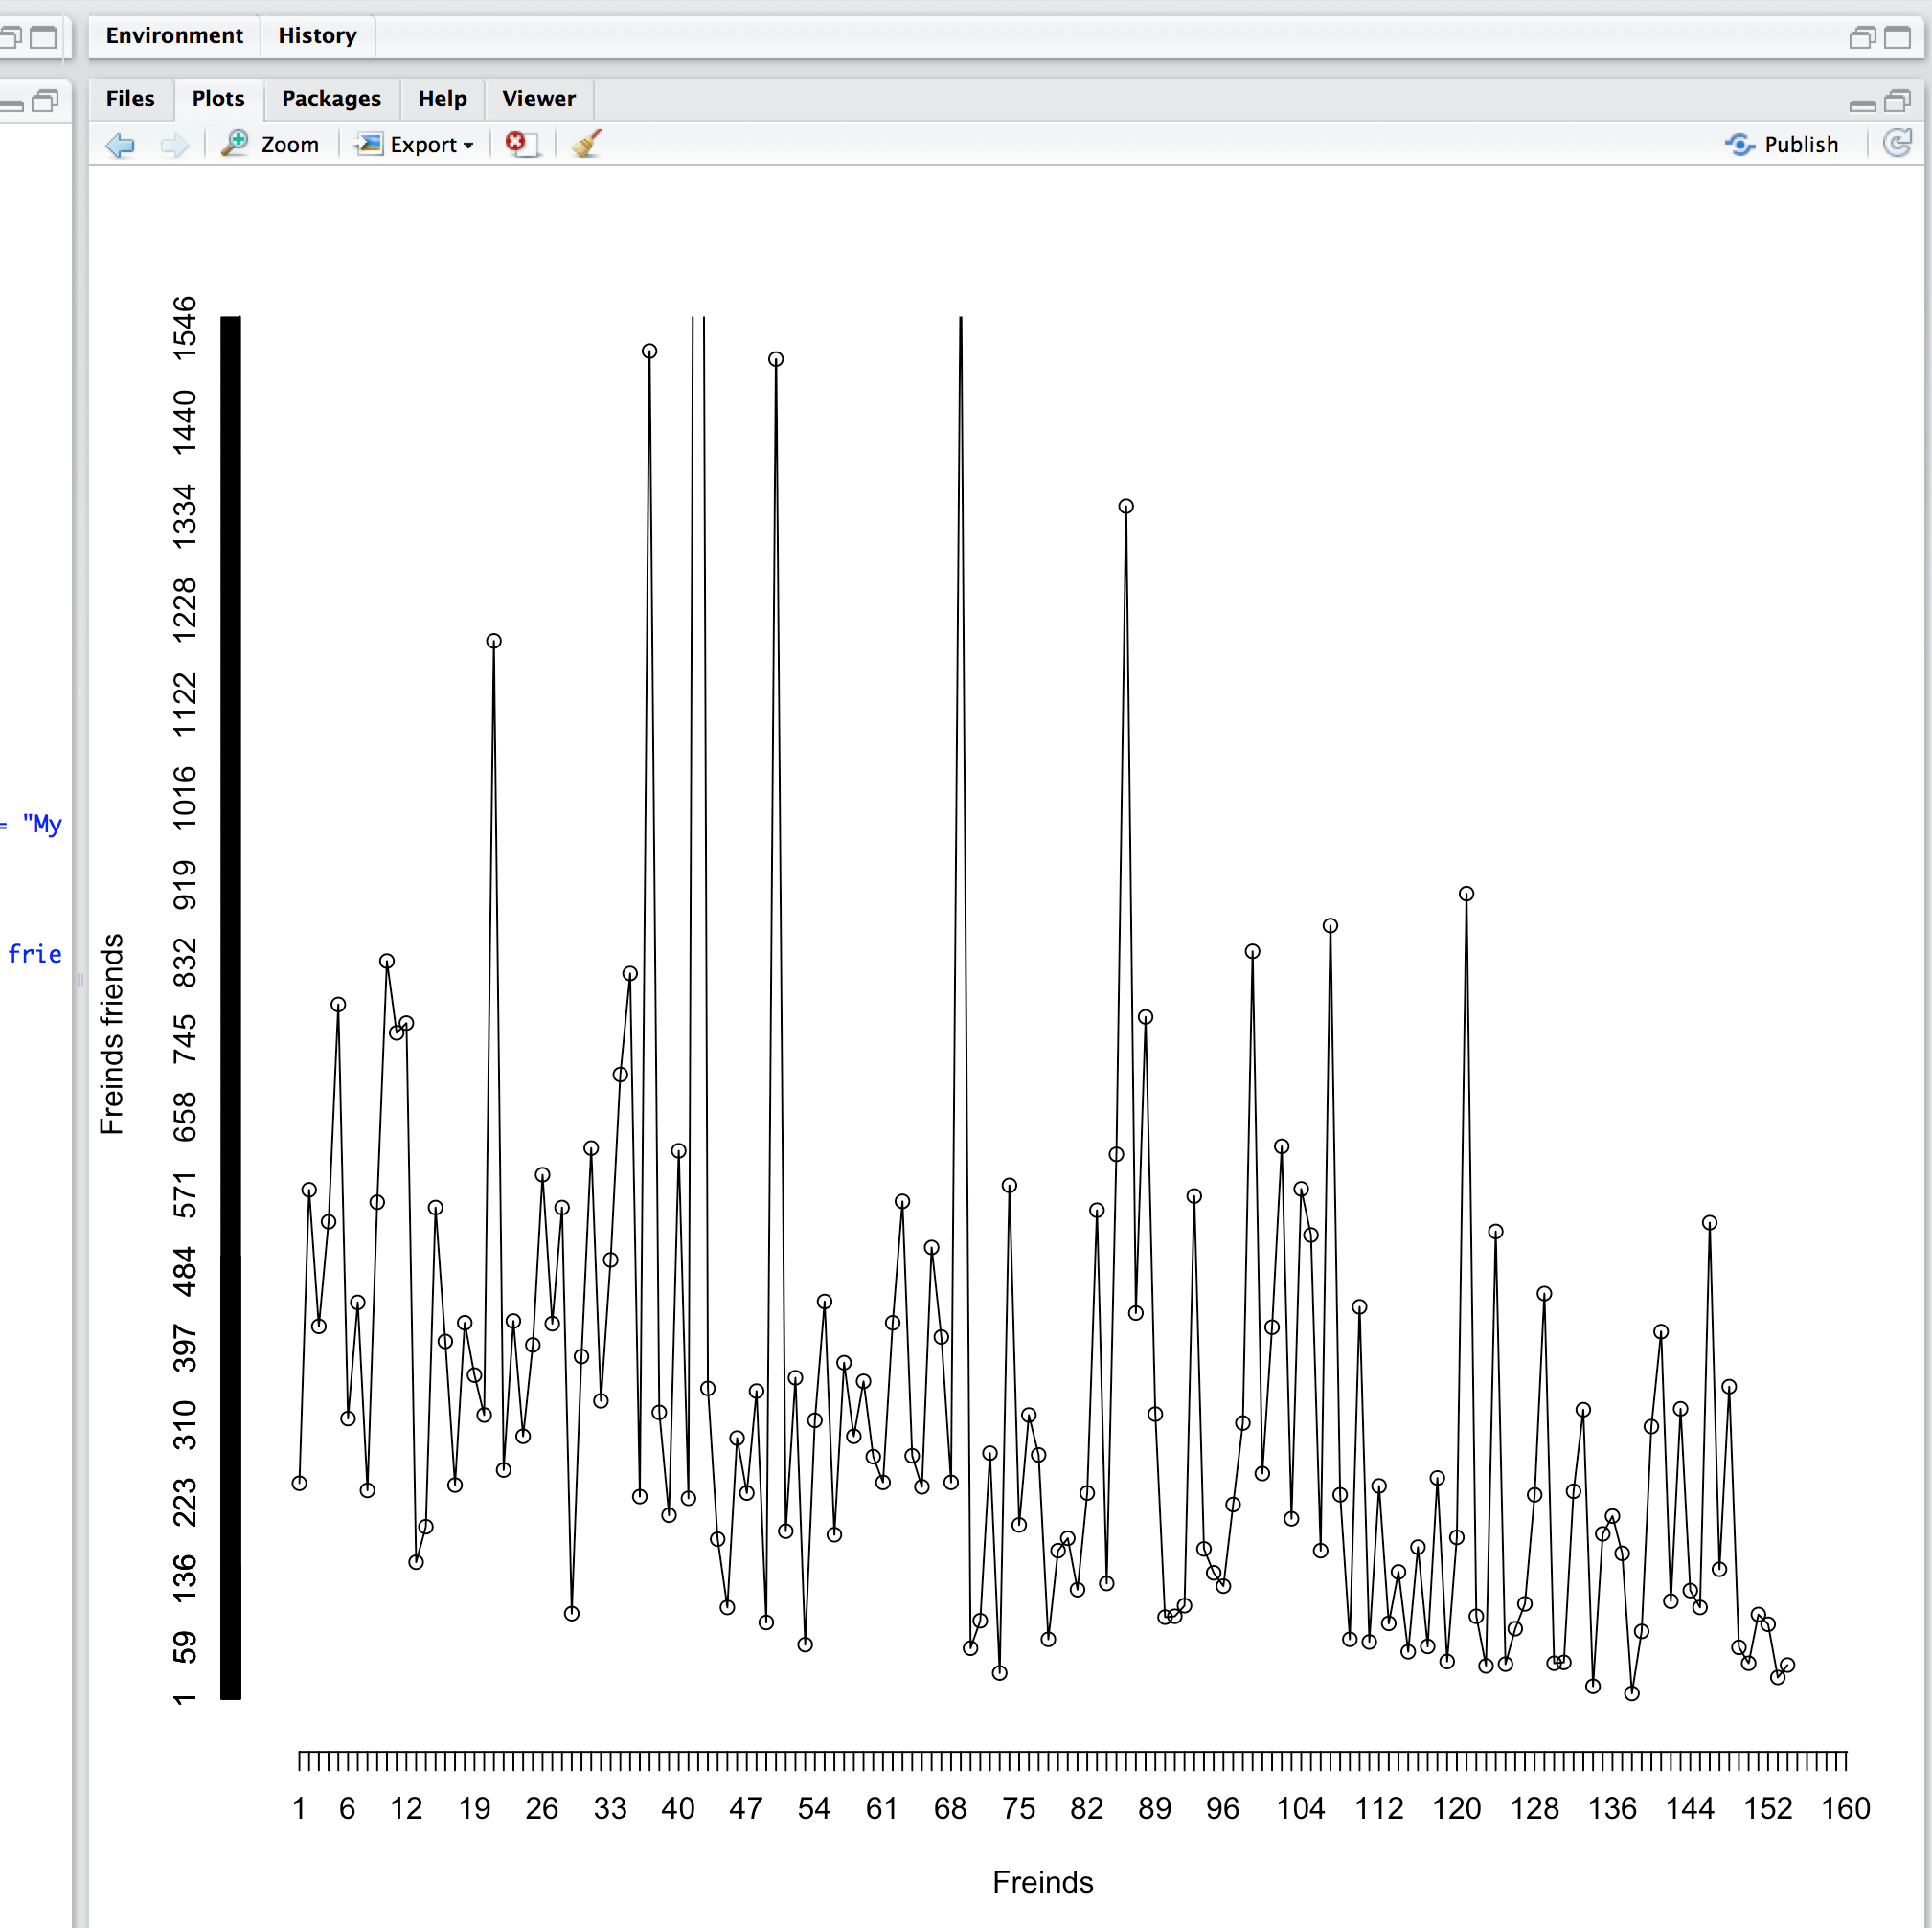
\includegraphics[scale=0.85]{Q2/fig1.png}
	\centerline{\textit{Figure 6: Output of q2.py at http://www.cs.odu.edu/\~{}mln/teaching/cs532-s16/test/pdfs.html
}}
\end{center}
\vspace*{5pt}
\begin{center}
	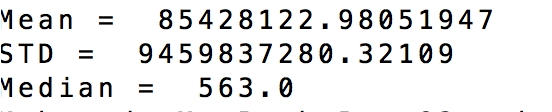
\includegraphics[scale=0.85]{Q2/fig2.png}
	\centerline{\textit{Figure 7: Output of q2.py at https://ws-dl.cs.odu.edu/Main/Pubs}}
\end{center}
\vspace*{5mm}
\begin{center}
	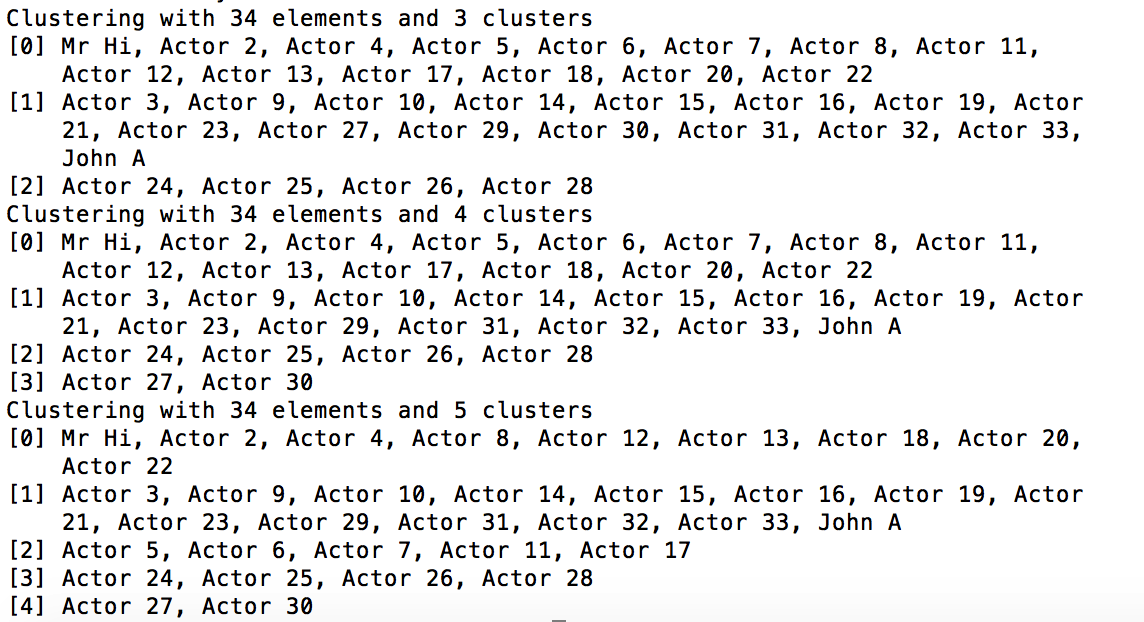
\includegraphics[scale=0.70]{Q2/fig3.png}
	\centerline{\textit{Figure 8: Output of q2.py at http://odu.edu/admission/graduate}}
\end{center}
Following python program $q2.py$, which accepts URL as argument and extracts PDF's from from the link:
\vspace*{1mm}

\begin{lstlisting}[frame = single,breaklines=true,numbers=left]
import sys
import requests
import validators
import locale
from urllib.parse import urlparse
from bs4 import BeautifulSoup

def main(url):
    print('\nExtracting all pdf links from: %s' % url)

    if requests.get(url).status_code != 200:
        print('\nURL not Found!\n')
        return
    page = requests.get(url).text
    url = 'http://' + urlparse(url).netloc
	
    soup = BeautifulSoup(page, 'html.parser')
    all_links = []
    for link in soup.find_all('a'):
        urls = link.get('href')
        if ((len(urls) > 6 and urls[:7].lower() != 'http://') 
        or len(urls) < 7) and urls[:8].lower() != 'https://':
            if urls[:2] == '//':
                urls = 'http:' + urls
            elif urls[0] != '/':    
                urls = url + '/' + urls
            else:
                urls = url + urls

        try:
            r = requests.get(urls)
            if 'Content-Type' in r.headers and 
            r.headers['Content-Type'] == 'application/pdf':
                if r.status_code == 200:
                    try:
                        all_links.append((urls, 
                        r.headers['Content-Length']))
                    except KeyError:
                        r.headers['Content-Length'] = '???'
                        all_links.append((urls, 
                        r.headers['Content-Length']))
        except requests.exceptions.SSLError:
            print('Couldn\'t open: %s. 
            URL requires authentication.' % urls)
        except requests.exceptions.ConnectionError:
            print('Couldn\'t open: %s. Connection refused.' % urls)
    print('\nList of all PDFs Links:')
    pdf_links = set(all_links)
    all_links = list(pdf_links)
    if len(all_links) > 0:
        for i in range(len(pdf_links)):
            if all_links[i][1] == '???':
                print('%s, File Size: %s bytes \n'
                 % (all_links[i][0], all_links[i][1]))
            else:
                print('%s, File Size: %s bytes \n' 
                % (all_links[i][0],                                  
                locale.format("%d", int(all_links[i][1]),
                grouping=True)))
    else:
        print('\nNo PDFs links for above URI.')
    return
if __name__ == '__main__':
    if len(sys.argv) != 2:
        print('\nUsage: python q2.py [url]')
        sys.exit(-1)
    if not validators.url(sys.argv[1]):
        print('URL is Invalid, Please try again')
        sys.exit(1)
    main(sys.argv[1])
    sys.exit(0)
\end{lstlisting}


\section{Problem 3}

\subsection{Question}
Compute the Kendall Tau\_b score for both lists (use \enquote{b} because
there will likely be tie values in the rankings).  Report both the
Tau value and the \enquote{p} value.\\
\\
See:\\ 
http://stackoverflow.com/questions/2557863/measures-of-association-in-r-kendalls-tau-b-and-tau-c\\
http://en.wikipedia.org/wiki/Kendall\_tau\_rank\_correlation\_coefficient\#Tau-b\\
http://en.wikipedia.org/wiki/Correlation\_and\_dependence\\



\subsection{Answer}
Using the Page Rank\cite{pagerank} Checker website to input each of the URIs found in the ten selected URIs from question 2 the results in Listing \ref{listing:pageranks} was determined.\\

\lstinputlisting[caption={page\_ranks file}, frame=none, stepnumber=0, label=listing:pageranks]{q3/page_ranks.txt}

In looking at the similarities and differences in the results of question 2 and question 3 it seems that page rank is unrelated to term frequency measurements. This is logical because the search term isn't taken as an input when calculating page rank. Also, finding page rank has a different goal than measuring search term relevance. It is used to objectively find which pages have a higher probability of a user randomly navigating to the page, which is unrelated to the content of the pages in the given set and is a function of the graph created by links contained in the pages of the set.

\newpage
\vspace*{5pt}
\bibliographystyle{unsrt}
\bibliography{a6}
\end{document}
